\documentclass[10pt]{article}
\usepackage[letterpaper,margin=1in]{geometry}
\usepackage[T1]{fontenc}
\usepackage{lmodern}
\usepackage{microtype}
\usepackage{amsmath}
\usepackage{graphicx}
\usepackage{booktabs}
\usepackage{tabularx}
\usepackage{xcolor}
\usepackage{tikz}
\usetikzlibrary{arrows.meta,positioning,fit,calc}
\usepackage[numbers,sort&compress]{natbib}
\usepackage{enumitem}
\usepackage{caption}
\usepackage[colorlinks=true,linkcolor=blue!50!black,citecolor=blue!50!black,urlcolor=blue!50!black]{hyperref}

\captionsetup{font=small,labelfont=bf}
\setlist{nosep,leftmargin=1.4em}
\definecolor{cblue}{HTML}{2a78d6}
\definecolor{corange}{HTML}{eb6834}
\definecolor{caqua}{HTML}{1baf7a}
\definecolor{ink2}{HTML}{52514e}

% generated by tools/make_tables.py
\newcommand{\Qval}{0.156}
\newcommand{\Qfull}{0.15605}
\newcommand{\Qlo}{0.144}
\newcommand{\Qhi}{0.168}
\newcommand{\Nepisodes}{1{,}000}
\newcommand{\Nsuccess}{37}
\newcommand{\SuccessRate}{3.7}
\newcommand{\Nnonzero}{71}
\newcommand{\Nzero}{29}
\newcommand{\Ntaskssuccess}{15}
\newcommand{\Nepnonzero}{364}
\newcommand{\WithinSD}{0.20}
\newcommand{\WithinSDnz}{0.237}
\newcommand{\Ntimeouts}{963}
\newcommand{\Spearman}{0.68}
\newcommand{\Pearson}{0.60}
\newcommand{\MeanExpected}{0.206}
\newcommand{\MeanRealized}{0.156}
\newcommand{\OptimismGap}{0.050}
\newcommand{\PredGain}{0.081}
\newcommand{\FallbackTasks}{63}
\newcommand{\StageOneTasks}{37}
\newcommand{\StageTwoTasks}{63}
\newcommand{\StageOneQ}{0.115}
\newcommand{\StageTwoQ}{0.180}
\newcommand{\StageOneE}{0.188}
\newcommand{\StageTwoE}{0.217}
\newcommand{\StageOneZeroOwn}{25}
\newcommand{\DevRollouts}{1{,}146}
\newcommand{\DevLabels}{36}
\newcommand{\DevEligible}{800}
\newcommand{\DevEligibleLabels}{28}
\newcommand{\ShareThirteen}{57}
\newcommand{\ShareThirteenElig}{47}
\newcommand{\PowerTwo}{1{,}568}
\newcommand{\PowerFive}{251}
\newcommand{\PowerTen}{63}
\newcommand{\PowerTwenty}{16}
\newcommand{\SelFive}{23}
\newcommand{\SelTen}{6}
\newcommand{\SelTwenty}{2}
\newcommand{\HistZero}{642}
\newcommand{\ReproAgree}{48}
\newcommand{\ReproTasks}{50}
\newcommand{\ReproRollouts}{411}
\newcommand{\ReproYmetz}{42}
\newcommand{\ReproNondefault}{8}
\newcommand{\ReproNondefaultAgree}{8}
\newcommand{\ReplayThirtyTwo}{716}
\newcommand{\ReplayTwenty}{277}
\newcommand{\ReplayZero}{7}
\newcommand{\DemoSpearman}{0.11}
\newcommand{\DepthZeroTasks}{25}
\newcommand{\DepthOneTasks}{46}
\newcommand{\DepthTwoTasks}{29}
\newcommand{\DepthZeroGap}{+1.5}
\newcommand{\DepthOneGap}{+4.1}
\newcommand{\DepthTwoGap}{-0.6}
\newcommand{\Kappa}{1.48}
\newcommand{\Sims}{300}
\newcommand{\SimStrictTrue}{0.186}
\newcommand{\SimStrictClaim}{0.188}
\newcommand{\SimStrictOpt}{+0.003}
\newcommand{\SimStrictRegret}{0.044}
\newcommand{\SimStrictRaw}{0.051}
\newcommand{\SimNaiveTrue}{0.191}
\newcommand{\SimNaiveClaim}{0.312}
\newcommand{\SimNaiveOpt}{+0.121}
\newcommand{\SimPostTrue}{0.192}
\newcommand{\SimPostOpt}{+0.003}
\newcommand{\SimPostRaw}{0.090}
\newcommand{\SimRefTrue}{0.063}
\newcommand{\SimOracle}{0.229}
\newcommand{\SimCostOfRules}{0.006}
\newcommand{\SimStrictEight}{0.201}
\newcommand{\SimNaiveEight}{0.215}
\newcommand{\ObsClaimed}{0.203}
\newcommand{\ObsRealized}{0.151}
\newcommand{\ObsOpt}{0.052}
\newcommand{\ObsRawGap}{0.062}
\newcommand{\ObsPct}{5}
\newcommand{\ObsLo}{0.152}
\newcommand{\ObsHi}{0.215}
\newcommand{\ExLevel}{0.179}
\newcommand{\ExLevelSd}{0.035}
\newcommand{\ExPrior}{0.170}
\newcommand{\ExPriorSd}{0.105}
\newcommand{\ExNoise}{0.091}
\newcommand{\ExPost}{0.152}
\newcommand{\ExPostSd}{0.100}

\newcommand{\Q}{\ensuremath{Q}}
\newcommand{\code}[1]{\texttt{#1}}
\makeatletter\newcommand{\rows}[1]{\@@input #1 }\makeatother

\title{\textbf{Policy Bank: Development-Selected Routing of Public Robot Policies for BEHAVIOR-1K}\\[4pt]
\large Team KANR technical report, 2026 BEHAVIOR Challenge}
\author{Keshav Balakrishna \and Abhijay Gangerapu \and Rithik Satarla\\[2pt]
\normalsize Team KANR (Independent)\\
\normalsize \url{https://github.com/FungousLand1941/policy-bank}}
\date{October 2026}

\begin{document}
\maketitle

\begin{abstract}
\noindent
The 2026 BEHAVIOR Challenge asks one system to complete 100 long-horizon household tasks in simulation. Rather than train a single generalist, we assemble a bank of ten public and lightly fine-tuned vision-language-action checkpoints and route each task to one of them. Routing uses only development instances: a hierarchical empirical-Bayes model combines public reference results, policy-level estimates paired against a reference policy, and our ledger of \DevRollouts{} development rollouts, and a conservative rule keeps the incumbent policy unless a challenger also beats it on shared instances. The frozen route was evaluated once on the ten public reporting instances of every task. It reaches $\Q=\Qval$ (95\% CI \Qlo--\Qhi) over \Nepisodes{} episodes, earning partial credit on \Nnonzero{} tasks but full success in only \Nsuccess{} episodes. Development estimates rank tasks well (Spearman \Spearman) yet are optimistic by \OptimismGap{} on average, and rollout noise (s.d.\ \WithinSD{} within a task) means telling apart two policies that differ by 0.05 takes about \PowerFive{} rollouts each. We release the route, all \Nepisodes{} metric files, the development ledger, a reimplementation of the selector that reproduces \ReproAgree{} of \ReproTasks{} stage-2 decisions, and a fail-stop serving layer for hidden evaluation.
\end{abstract}

\section{Introduction}

BEHAVIOR-1K~\cite{li2024behavior1k,li2023behavior1k} defines everyday household activities in realistic simulation, and its 2026 challenge~\cite{behavior2026challenge} scores a single submission on 100 of them. Each task is long: the mean human demonstration runs from about one to fifteen minutes, and an episode ends when the goal is reached or when the robot has used 1.5 times the mean demonstration length. Partial credit counts the fraction of goal conditions satisfied, and the challenge score \Q{} averages it over tasks.

By the 2026 challenge several strong public checkpoints existed, each built on the $\pi_0$/$\pi_{0.5}$ vision-language-action family~\cite{black2024pi0,pi05,openpi}: the Comet team's 2025 models~\cite{bai2025comet}, the four checkpoints of the 2025 winning solution~\cite{larchenko2025task}, continuations of these on the 2026 demonstrations, and community specialists fine-tuned for a handful of tasks. They differ sharply by task. A checkpoint that wins one task may score zero on the next. With a fixed compute budget, the question we study is practical: \emph{which checkpoint should run each task, decided only from development data, without fooling ourselves with noise?}

This is an algorithm-selection problem~\cite{rice1976algorithm} with three complications. First, evidence is scarce: a single rollout runs for up to 22 simulated minutes, and longer in wall-clock time, so most (task, policy) pairs get one to three development rollouts. Second, rollouts are noisy: the same policy on the same task scores 0 on one instance and 1 on the next. Third, choosing the best-looking option from noisy estimates is optimistically biased (the optimizer's curse~\cite{smith2006optimizer}). Our approach treats routing as shrinkage estimation~\cite{efron1975stein}. Every (task, policy) pair gets an informative prior, development rollouts update it, and a policy displaces the incumbent only when several conservative conditions agree.

\paragraph{Contributions.}
\begin{enumerate}
\item A \emph{policy bank} of ten checkpoints, each served with its native adapter, and a frozen per-task route chosen without looking at reported instances (Sections~\ref{sec:bank}--\ref{sec:routing}).
\item A development-selection method: transfer priors from public reference results, paired policy-level priors where none exist, conjugate updates, and strict switching rules (Section~\ref{sec:routing}).
\item An audited evaluation: $\Q=\Qval$ [\Qlo, \Qhi] on \Nepisodes{} unchanged episodes, with score-blind duplicate handling and every deviation disclosed (Sections~\ref{sec:protocol}--\ref{sec:results}).
\item An analysis of calibration, noise and statistical power that explains why per-task routing gains are hard to verify at challenge scale (Section~\ref{sec:analysis}).
\item A fail-stop serving layer for hidden evaluation and an open release of code, data and route (Section~\ref{sec:serving}).
\end{enumerate}

\section{Related work}

\paragraph{Vision-language-action policies.} $\pi_0$~\cite{black2024pi0} attaches a flow-matching action expert to a PaliGemma vision-language backbone~\cite{beyer2024paligemma}, and $\pi_{0.5}$~\cite{pi05} adds co-training for open-world generalization. All checkpoints in our bank descend from this line through OpenPI~\cite{openpi}.

\paragraph{BEHAVIOR solutions.} The 2025 winning solution~\cite{larchenko2025task} adapted $\pi_{0.5}$ with correlated-noise flow matching, stage tracking and task-specific correction rules, reaching \Q{}$\approx$0.26 on 50 tasks. Openpi Comet~\cite{bai2025comet}, second in 2025, studied pre-training and post-training recipes at scale. We train almost nothing ourselves. Our contribution is to select among such models and to measure the result carefully.

\paragraph{Selection under noise.} Per-instance algorithm selection~\cite{rice1976algorithm} picks the best solver for each input. Empirical Bayes and Stein shrinkage~\cite{efron1975stein} improve many noisy means at once by borrowing strength across them, and the optimizer's curse~\cite{smith2006optimizer} predicts that the chosen option will disappoint on average. Our results show this effect directly (Section~\ref{sec:calibration}).

\section{Problem setup}
\label{sec:setup}

\paragraph{Tasks and scoring.} Each of the 100 tasks $t$ has a goal written in BDDL. An episode ends at success or when the simulator step count reaches 1.5 times the mean demonstration length for $t$. Its score $q\in[0,1]$ is the fraction of goal conditions satisfied at the end, with $q=1$ exactly at success. With $I=\{301,\dots,310\}$ the reporting instances,
\begin{equation}
\Q=\frac{1}{100}\sum_{t=1}^{100}\frac{1}{|I|}\sum_{i\in I} q_{t,i},
\end{equation}
where a missing cell counts as zero. Instances 311--320 are reserved for development; the organizers evaluate submitted containers on hidden instances 321--340.

\paragraph{Robot and interface.} The robot is a wheeled bimanual R1Pro. A policy receives head and wrist RGB-D images, a 61-dimensional proprioceptive vector and the task identity. It returns 23-dimensional actions over a websocket, optionally several per query. Hidden evaluation requires an average of at least one simulator frame per second including inference, at most 600\,s per query, and a single 24\,GB GPU per policy.

\paragraph{Rules we imposed on ourselves.} Policies use only onboard sensors at test time. Every routing decision uses development instances only, every reported cell is run once, and a route is frozen and hashed before reported evaluation of the affected tasks begins.

\section{The policy bank}
\label{sec:bank}

Table~\ref{tab:bank} lists the ten routed checkpoints with their exact sources. They fall into three families.
\textbf{Comet} ($\pi_{0.5}$, 32-step action chunks): the released \code{pt50} and \code{pt12} checkpoints~\cite{bai2025comet,comethf}; a public continuation of \code{pt50} on the 2026 demonstrations by ymetz (step 9999); and \code{s150997}, our own continued training of \code{pt50} on the 2026 demonstrations of all 100 tasks.
\textbf{Winner} (re-planning every 20 steps): the four checkpoints of the 2025 winning solution~\cite{larchenko2025task,winnerhf}, served with their native wrapper and correction rules.
\textbf{Winner-format specialists}: two community models fine-tuned for a few 2026 tasks, one covering tasks 54, 56, 77 and 98 and one released for tasks 90, 91, 93, 96 and 97.

Every checkpoint runs behind its own native adapter: prompts, image preprocessing, normalization statistics, action representation and replay horizon are those of its publisher. We do not merge weights or ensemble actions; the bank is a lookup table from task to checkpoint. Our development ledger also covers \DevLabels{} policy labels in total, including other checkpoint steps, a third-party 100-task model, action-search variants, time compression, gripper-correction add-ons and a modified robot configuration. None of these entered the route.

\begin{table}[t]
\centering\small
\caption{The routed checkpoints. Revisions are Hugging Face commit prefixes. No weights are redistributed with this report.}
\label{tab:bank}
\begin{tabular}{@{}lll@{}}
\toprule
Policy & Source (repository/subfolder) & Revision \\
\midrule
\rows{generated/bank.tex}
\bottomrule
\end{tabular}
\end{table}

\section{Development-selected routing}
\label{sec:routing}

\subsection{Model}
Let $\theta_{tp}$ be the expected score of policy $p$ on task $t$. We place a Gaussian prior $\theta_{tp}\sim\mathcal N(\mu_{tp},\tau_{tp}^2)$ and treat each development rollout as $y_{tpk}\sim\mathcal N(\theta_{tp},\sigma_p^2)$. With $n$ rollouts of mean $\bar y$, the posterior is
\begin{equation}
\theta_{tp}\mid y \sim \mathcal N\!\left(\frac{\mu_{tp}/\tau_{tp}^2 + n\bar y/\sigma_p^2}{1/\tau_{tp}^2+n/\sigma_p^2},\;\Big(\frac{1}{\tau_{tp}^2}+\frac{n}{\sigma_p^2}\Big)^{-1}\right).
\label{eq:post}
\end{equation}
The rollout variance $\sigma_p^2$ is the pooled within-task variance of $p$'s development rollouts, shrunk toward a default with a few pseudo-degrees of freedom. Rollout scores are bounded and often bimodal, so the Gaussian is an approximation. Its job is to weigh a prior against a handful of rollouts, not to model $q$ exactly.

\subsection{Priors where public reference results exist (tasks 0--49)}
For the first 50 tasks, the 2025 challenge and its participants published per-task results for the Comet and winner checkpoints. These results come from a different simulator setup and different instances, so we scale them by a transfer factor $\gamma$:
\begin{equation}
\mu_{tp}=\gamma_f\, r_{tp},\qquad \tau_{tp}^2=(r_{tp}\,s_{\gamma})^2+b^2,
\end{equation}
where $r_{tp}$ is the reference score, $s_\gamma$ the factor's uncertainty and $b\approx0.09$ a floor for task-specific deviations. For \code{pt50}, $\gamma$ is estimated as the ratio of our development means to the reference over the other tasks (leave-one-task-out), giving $0.55\pm0.09$. For the winner family we fixed $\gamma=0.81\pm0.10$ before stage 2; an empirical-Bayes estimate from 31 winner development rollouts gave $0.69\pm0.11$.

\subsection{Priors without reference results (tasks 50--99)}
Tasks 50--99 are new in 2026, so no public per-task results exist. We estimate a \emph{policy level} instead. The reference policy \code{s150997} has development rollouts on almost every task, so its level $\ell_{\mathrm{ref}}$ is the mean of its per-task means over the other tasks. A candidate's level is the reference level plus its mean paired difference on the tasks both have run:
\begin{equation}
\ell_p=\ell_{\mathrm{ref}}+\frac{1}{|S_p|}\sum_{u\in S_p}\big(\bar y_{up}-\bar y_{u,\mathrm{ref}}\big),\qquad S_p=\{u\neq t:\ \text{both ran }u\}.
\end{equation}
Pairing removes much of the between-task variation, because candidates are compared on the same tasks. Each level is combined with its family's other members, or with a weak hyperprior $\mathcal N(0.1,0.1^2)$, and widened by a between-task standard deviation of 0.1 to give $(\mu_{tp},\tau_{tp})$. For example, the ymetz continuation has a level of $0.184\pm0.048$ and a task prior of $0.184\pm0.111$. One development rollout scoring 0 moves this prior to a posterior mean of $0.160$, as Eq.~\eqref{eq:post} predicts.

\subsection{Switching rules}
A posterior ranking alone would chase noise, so a challenger must pass every rule below:
\begin{enumerate}
\item \textbf{Own evidence}: at least two of its own development rollouts on the task (tasks 0--49).
\item \textbf{Development guard}: it must also beat the incumbent on the development instances both ran (at least two shared instances), not only in posterior mean.
\item \textbf{Margin}: posterior gain of at least 0.01 over the incumbent.
\item \textbf{Veto}: it is rejected if it scored 0 on every instance where the incumbent scored above 0.1.
\item \textbf{Scope}: a specialist is a candidate only on tasks where it has its own development rollouts, and only if it has at least two rollouts in total.
\item \textbf{One checkpoint per family}: when two checkpoints of one family win different tasks, the one with the larger summed posterior gain takes both. This keeps the number of serving images small.
\end{enumerate}
On tasks 0--49 every challenger must pass all rules. On tasks 50--99 the incumbent is the weak reference policy and the highest eligible posterior wins after the veto, scope and family rules.

\subsection{Two-stage freeze}
\begin{figure}[t]
\centering
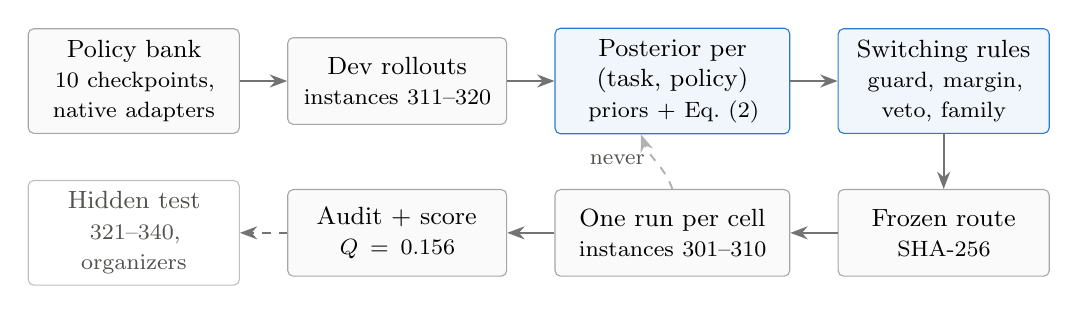
\begin{tikzpicture}[
  font=\small, node distance=4mm and 6mm,
  box/.style={draw=black!35, rounded corners=2pt, align=center, inner sep=4pt, fill=black!2, minimum height=11mm},
  hot/.style={box, draw=cblue, fill=cblue!7},
  arr/.style={-{Stealth[length=2.2mm]}, black!55, line width=0.7pt}]
\node[box, text width=24mm] (bank) {Policy bank\\{\footnotesize 10 checkpoints, native adapters}};
\node[box, right=of bank, text width=25mm] (dev) {Dev rollouts\\{\footnotesize instances 311--320}};
\node[hot, right=of dev, text width=27mm] (post) {Posterior per (task, policy)\\{\footnotesize priors + Eq.~(2)}};
\node[hot, right=of post, text width=24mm] (rules) {Switching rules\\{\footnotesize guard, margin, veto, family}};
\node[box, below=7mm of rules, text width=24mm] (route) {Frozen route\\{\footnotesize SHA-256}};
\node[box, left=of route, text width=27mm] (eval) {One run per cell\\{\footnotesize instances 301--310}};
\node[box, left=of eval, text width=25mm] (audit) {Audit + score\\{\footnotesize $Q=\Qval$}};
\node[box, left=of audit, text width=24mm, draw=black!25, fill=white, text=ink2] (hidden) {Hidden test\\{\footnotesize 321--340, organizers}};
\draw[arr] (bank) -- (dev);
\draw[arr] (dev) -- (post);
\draw[arr] (post) -- (rules);
\draw[arr] (rules) -- (route);
\draw[arr] (route) -- (eval);
\draw[arr] (eval) -- (audit);
\draw[arr, dashed] (audit) -- (hidden);
\draw[arr, dashed, black!30] (eval.north) to[out=110, in=-70] node[pos=0.55, left, font=\footnotesize, text=ink2]{never} ($(post.south)+(-0.4,0)$);
\end{tikzpicture}
\caption{Development-selected routing. Reported instances (301--310) are never an input to a routing decision. The route is frozen and hashed before reported evaluation.}
\label{fig:pipeline}
\end{figure}

Evaluation compute was the binding constraint, so routing was frozen in two stages (Figure~\ref{fig:pipeline}). Stage~1 fixed the \StageOneTasks{} tasks whose choice was already settled by priors and early development evidence, and their reported runs began on 11 October. The other \StageTwoTasks{} tasks were deferred while development rollouts accumulated. Their route was written from 860 development rollouts and frozen at 12:54 UTC on 13 October. Every reported episode of these tasks ran under its stage-2 entry; the earliest finished at 13:10 UTC. Each deferred task also carried a fallback policy, to be used if its stage-2 entry had not arrived by a deadline. The route tables are identified by SHA-256 in the release, and every reported episode was produced by its task's routed policy (checked in the test suite).

\section{Evaluation protocol}
\label{sec:protocol}

\paragraph{Infrastructure.} Reported and development runs used TACC Stampede3 nodes with two NVIDIA RTX PRO 6000 Blackwell GPUs, running Isaac Sim 6.0.1 inside the organizers' container image. Isaac Sim 5.1, the version prescribed for hidden evaluation, crashed with the cluster's GPU driver; the organizers allowed Isaac Sim 6 for public results. Each simulator connects to its own policy server, because one native server keeps a single action plan for all connections. Camera inputs use the full-resolution RGB-D wrapper. A paired development comparison over 38 cells found 224-pixel inputs worse by 0.061 on average, so we kept full resolution. Over the project we used roughly 1,500 documented allocated GPU-hours, including idle and failed allocations.

\paragraph{Integrity rules.} The reporting set contains exactly one unchanged metrics file per (task, instance), 1,000 in total, each identified by SHA-256. Infrastructure retries produced two completed duplicate cells. In both we kept the attempt that \emph{finished first}, regardless of its score: \code{spraying\_for\_bugs}/307 (kept 0.5, later 0.0) and \code{cook\_brussels\_sprouts}/303 (kept 0.0, later 0.0). Logs show the later attempt started after the kept one ended. No development rerun or later experiment was merged into the reporting set.

\paragraph{Execution details.} Comet-family policies replay 32 actions per query and winner-format policies 20. In the reporting set, \ReplayThirtyTwo{} episodes ran with replay 32, \ReplayTwenty{} with replay 20, and \ReplayZero{} came from a recovery pass that replays 0 actions (one query per control step). We report those seven unchanged. The copy of the organizers' scorer bundled with the simulator divides by a 20-instance public pool and returns 0.078 on our files. The published reporting contract uses ten instances, and the same unmodified functions with that denominator give \Qfull. We changed neither the scorer nor the files.

\section{Results}
\label{sec:results}

\begin{table}[t]
\centering\small
\caption{Headline results on the reporting instances (Isaac Sim 6.0.1). The confidence interval resamples instances within each task (10{,}000 bootstrap draws). This is a self-evaluated public score, not a hidden-test score.}
\label{tab:headline}
\begin{tabular}{@{}lr@{}}
\toprule
Challenge score \Q{} (95\% CI) & \Qval{} (\Qlo--\Qhi) \\
Episodes / tasks & \Nepisodes{} / 100 \\
Full successes & \Nsuccess{} (\SuccessRate\%) in \Ntaskssuccess{} tasks \\
Tasks with partial credit ($\bar q>0$) & \Nnonzero{} \\
Tasks scoring zero on all ten instances & \Nzero{} \\
Episodes with $q>0$ & \Nepnonzero{} \\
\bottomrule
\end{tabular}
\end{table}

Table~\ref{tab:headline} summarizes the run. The score is mostly partial credit: \Nepnonzero{} episodes satisfy at least one goal condition, but only \Nsuccess{} finish their task. All \Ntimeouts{} unsuccessful episodes ran to the step cap. None ended early for any other reason.

\begin{figure}[t]
\centering
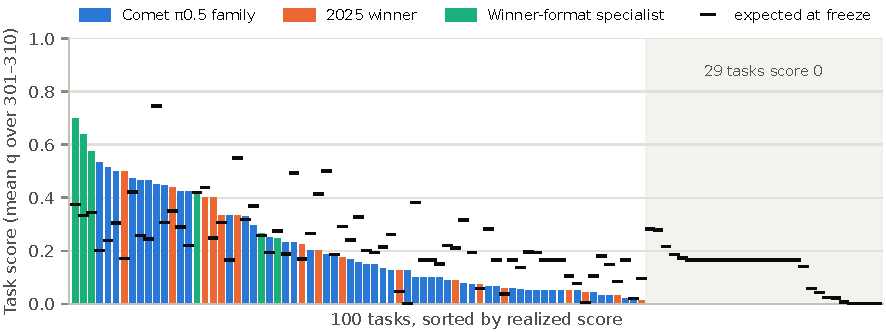
\includegraphics[width=\linewidth]{figures/tasks.pdf}
\caption{Realized score per task (bars, colored by policy family) against the posterior expectation at freeze (ticks), sorted by realized score. Twenty-nine tasks score zero on all ten instances.}
\label{fig:tasks}
\end{figure}

Figure~\ref{fig:tasks} shows the per-task picture. The highest-scoring tasks are served by the four-task specialist and the strongest Comet and winner checkpoints (Table~\ref{tab:top}). Twenty-nine tasks score zero on all ten instances. Their demonstrations are not longer than average (mean 319\,s against 352\,s over all tasks). On 23 of them no development rollout of any policy scored above zero either. On the other six, at least one development rollout made progress, in four cases a full success, which shows how far a single development rollout can mislead.

\begin{table}[t]
\centering\small
\caption{The ten highest-scoring tasks.}
\label{tab:top}
\begin{tabular}{@{}rllrrr@{}}
\toprule
ID & Task & Policy & Expected & Realized & Successes \\
\midrule
\rows{generated/toptasks.tex}
\bottomrule
\end{tabular}
\end{table}

\begin{table}[t]
\centering\small
\caption{Per-policy outcome. ``Expected'' is the mean posterior expectation over the policy's routed tasks at freeze. ``Task points'' is the sum of its tasks' scores, so the column sums to $100\,\Q$.}
\label{tab:policies}
\begin{tabular}{@{}llrrrrrr@{}}
\toprule
Policy & Family & Replay & Tasks & Expected & Realized & Successes & Task points \\
\midrule
\rows{generated/policies.tex}
\bottomrule
\end{tabular}
\end{table}

\begin{figure}[t]
\centering
\begin{minipage}[t]{0.49\linewidth}\centering
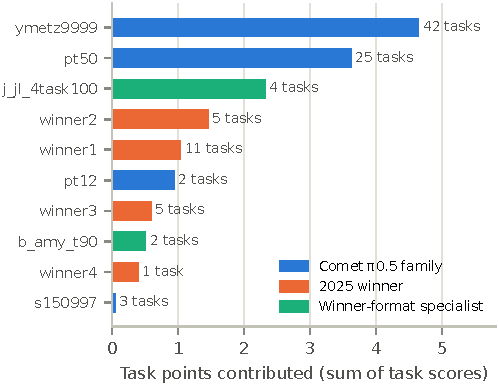
\includegraphics[width=\linewidth]{figures/policies.pdf}
\caption{Contribution of each routed policy to \Q{}, in task points.}
\label{fig:policies}
\end{minipage}\hfill
\begin{minipage}[t]{0.49\linewidth}\centering
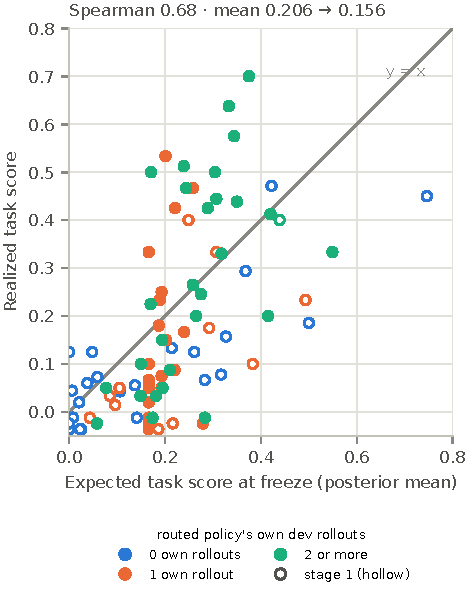
\includegraphics[width=\linewidth]{figures/calibration.pdf}
\caption{Expected (posterior at freeze) versus realized task score. Points below the diagonal disappointed.}
\label{fig:calibration}
\end{minipage}
\end{figure}

\paragraph{Per policy.} Table~\ref{tab:policies} and Figure~\ref{fig:policies} break the score down by policy. The ymetz continuation of \code{pt50} carries 42 of the 50 new tasks and contributes the most task points. Its per-task average (0.111) is modest, but it beat our own continued training on development pairs. The four-task specialist is the standout: 0.581 on its four tasks, eleven of the \Nsuccess{} successes, and well above its expectation. The two \code{pt12} tasks and \code{winner4}'s microwave-popcorn task also score high. Our own checkpoint \code{s150997} kept only three tasks and earned almost nothing on them, which is consistent with its low development level.

\paragraph{Per scene.} Scores range from 0.30 on the five \code{hotel\_suite\_large} tasks to 0.075 on the ten upper-floor tasks of \code{house\_double\_floor} (Table~\ref{tab:scenes}). Mean demonstration length is only weakly related to task score (Spearman \DemoSpearman).

\begin{table}[t]
\centering\small
\caption{Mean task score by scene.}
\label{tab:scenes}
\begin{tabular}{@{}lrr@{}}
\toprule
Scene & Tasks & Mean task score \\
\midrule
\rows{generated/scenes.tex}
\bottomrule
\end{tabular}
\end{table}

\section{Analysis}
\label{sec:analysis}

\subsection{Calibration and the optimizer's curse}
\label{sec:calibration}
Figure~\ref{fig:calibration} compares each task's posterior expectation at freeze with its realized score. The ranking holds up: Spearman \Spearman{} and Pearson \Pearson{} across the 100 tasks. The level does not. The mean expectation was \MeanExpected{}, the mean realization \MeanRealized{}. This is the optimizer's curse~\cite{smith2006optimizer}: we chose, per task, the policy whose estimate looked best, so on average its estimate was too high. Shrinkage reduces the bias but cannot remove it with this little data.

The bias differs by stage. Stage-1 tasks realized \StageOneQ{} against an expected \StageOneE{} (ratio \StageOneRatio). Stage-2 tasks realized \StageTwoQ{} against \StageTwoE{} (ratio \StageTwoRatio). Stage-1 priors leaned on 2025 reference results transferred to a new simulator and new instances, so they carried the most optimism. Stage-2 priors were built from our own paired development rollouts, under the same setup as the reported run.

\subsection{Rollout noise and statistical power}
\label{sec:noise}
\begin{figure}[t]
\centering
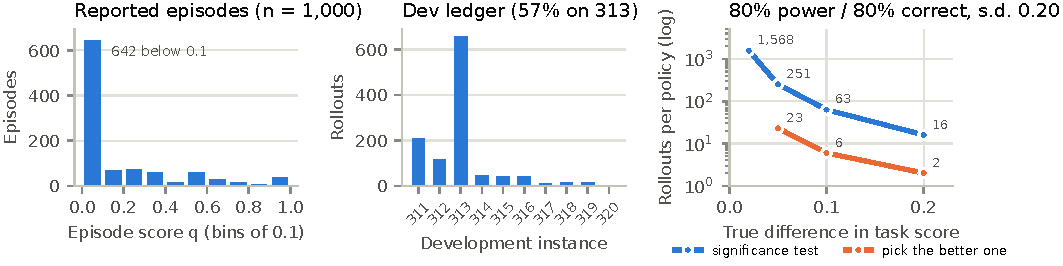
\includegraphics[width=\linewidth]{figures/noise.pdf}
\caption{Left: episode scores pile up at zero. Middle: development rollouts concentrated on one instance. Right: rollouts per policy needed to detect a given difference in task score at 80\% power ($\alpha=0.05$, unpaired), using the within-task standard deviation of the reported run.}
\label{fig:noise}
\end{figure}
Within a task, reported episode scores have a standard deviation of \WithinSD{}, and \HistZero{} of \Nepisodes{} episodes score below 0.1 (Figure~\ref{fig:noise}). Telling apart two policies whose true task scores differ by 0.05 takes about \PowerFive{} rollouts per policy at 80\% power; a difference of 0.10 takes \PowerTen{} and a difference of 0.20 takes \PowerTwenty. Our whole ledger has \DevRollouts{} rollouts over \DevLabels{} policy labels. Of the 404 (task, policy) cells eligible for selection, 198 have a single rollout and 91\% have at most three, and \ShareThirteen\% of all development rollouts used instance 313. In this regime only large differences can be resolved per task. The priors and paired levels in Section~\ref{sec:routing} carry most of the information, and the switching rules exist to stop single lucky rollouts from changing the route. Before the deadline we estimated that all 54 remaining per-task switch proposals together were worth about $+0.007$ \Q{}, too little to justify a rerun.

\subsection{Reproducing the selection}
Our package contains a clean reimplementation of the selector (\code{policybank.selection}). Run on the released development ledger, restricted to rollouts finished before the stage-2 freeze (\ReproRollouts{} rollouts on tasks 50--99), it reproduces \ReproAgree{} of the \ReproTasks{} stage-2 decisions for those tasks. In both disagreements (tasks 70 and 87) the reimplementation keeps the reference policy where the frozen route chose the ymetz continuation. The frozen route came from the original pipeline, whose development table and filtering differ slightly from the released ledger. We do not reproduce tasks 0--49 because their priors depend on third-party reference tables that we do not redistribute.

\subsection{What did not make the route}
Several ideas were tested on development instances and rejected, or never reached a decisive comparison: replaying demonstrations on near-duplicate test scenes (0 of 14 twin-test episodes succeeded, mostly from grasp misses), time-compressed action playback, gripper-correction add-ons for the Comet family, sampled action search, a modified robot configuration, 224-pixel camera inputs, and a third-party 100-task model whose port to our serving stack never produced enough nonzero development rollouts to rule out a porting error. Given the power analysis above, ``rejected'' often means ``not shown to help'' rather than ``shown not to help.''

\section{Serving for hidden evaluation}
\label{sec:serving}
Hidden evaluation runs the submitted containers on the organizers' hardware. We package one image per routed policy, and each container is bound at runtime to a single task. The server enforces a strict contract on every frame and fails closed:
\begin{itemize}
\item one task per container and one evaluator session at a time (a second connection is refused with close code 1013);
\item batches of 1--10 environments with a fixed shape until reset; a reset clears the action queues before the next action;
\item a single global transport chunk $K=4$ that divides both native replay lengths (32 and 20), so the chunked action stream is identical to the native receding-horizon stream (tested for both lengths);
\item malformed frames, wrong shapes, nonfinite actions, model exceptions and per-query timeouts (550\,s, below the 600\,s rule) close the connection with code 1011 and stop the process; there is no retry, no substitute action, no fallback checkpoint and no automatic restart, because a fabricated action could turn a fault into a silent wrong result.
\end{itemize}
The release contains this layer (codec, contract, chunk executor, server and client) with integration tests against a scripted policy. In the original packaging, all ten native models passed startup, warm-up and synthetic-input batch-1 and batch-10 protocol tests on an RTX~3090 as an unprivileged user; the longest batch-10 query took 3.38\,s and sampled GPU memory stayed below 9\,GB. A separate strict-isolation test, which restricted file writes and outbound connections, failed for all ten because CUDA reported no visible GPU. We have not established whether the isolation harness or the images cause this. We have not completed full simulator episodes under Isaac Sim 5.1 at the required one frame per second on the organizers' GPU class, so hidden-evaluation readiness remains unverified.

\section{Limitations and disclosures}
\begin{itemize}
\item \Q{} is a self-evaluated score on public reporting instances produced with Isaac Sim 6.0.1, not a hidden-test score or a prediction of placement. Hidden evaluation uses Isaac Sim 5.1, and simulator differences may shift scores.
\item Development evidence is thin and concentrated on a few instances. Routes for individual tasks are therefore uncertain even when the aggregate ranking is informative.
\item Two duplicate cells were resolved by completion order, and seven episodes used a different replay length. Both are disclosed above and left unchanged.
\item We do not redistribute model weights. The publishers of the winner checkpoints and the four-task specialist declare Apache-2.0 at the pinned revisions. The ymetz card defers to its base checkpoint's terms. We did not find an explicit licence for the separately hosted Comet weights or for the specialist used on tasks 96--97. Credits are attribution, not a licence grant.
\item The released selector reproduces the frozen stage-2 decisions closely but not exactly, and the stage-1 priors depend on reference tables we do not redistribute.
\end{itemize}

\section{Conclusion}
A bank of public checkpoints, routed per task from development data alone, reached $\Q=\Qval$ on the public reporting instances of the 2026 BEHAVIOR Challenge. Most of the score comes from partial credit, and a third of the tasks remain out of reach for every checkpoint we could run. The more transferable lesson concerns measurement. At ten-instance scale with per-rollout noise of \WithinSD{}, the best-looking choice is reliably optimistic and per-task gains below about 0.1 cannot be verified. Priors that borrow strength across tasks and policies, conservative switching rules, a frozen route, and score-blind bookkeeping are what make the reported number trustworthy. Code, data and the route are available at \url{https://github.com/FungousLand1941/policy-bank}.

\section*{Acknowledgments}
We thank the authors of every checkpoint in the bank: Team Comet, Ilia Larchenko, Gleb Zarin and Akash Karnatak, ymetz, JackLiu0406 and amyjia1212. We also thank Physical Intelligence for OpenPI and Google for PaliGemma, the Stanford BEHAVIOR-1K team for the benchmark, the challenge and the demonstrations, and the Texas Advanced Computing Center for Stampede3. Parts of the evaluation tooling and of this report's analysis code were written with AI coding assistants. Every number in this report is recomputed from the released data by the released code.

\small
\bibliographystyle{plainnat}
\bibliography{refs}

\end{document}
